\documentclass[11pt,a4paper]{article}

% ---- Язык и шрифты (Cyrillic через XeLaTeX) --------------------------------
\usepackage{fontspec}
\usepackage{polyglossia}
\setdefaultlanguage{russian}
\setotherlanguage{english}
\setmainfont{DejaVu Serif}
\setsansfont{DejaVu Sans}
\setmonofont{DejaVu Sans Mono}[Scale=0.80]

% ---- Геометрия и оформление -------------------------------------------------
\usepackage[a4paper,margin=2.2cm,headheight=14pt]{geometry}
\usepackage{amsmath}
\usepackage{graphicx}
\usepackage{float}
\usepackage{xcolor}
\usepackage{listings}
\usepackage{booktabs}
\usepackage{longtable}
\usepackage{array}
\usepackage{enumitem}
\usepackage{titlesec}
\usepackage{fancyhdr}
\usepackage[hidelinks,unicode]{hyperref}
\usepackage{tcolorbox}
\tcbuselibrary{skins,breakable}

\definecolor{accent}{RGB}{20,90,150}
\definecolor{accent2}{RGB}{190,90,20}
\definecolor{codebg}{RGB}{247,247,248}
\definecolor{codekw}{RGB}{0,0,170}
\definecolor{codecm}{RGB}{0,128,0}
\definecolor{codestr}{RGB}{163,21,21}
\definecolor{rulegray}{RGB}{180,180,180}

\titleformat{\section}{\Large\bfseries\color{accent}}{\thesection}{0.6em}{}
\titleformat{\subsection}{\large\bfseries\color{accent!80!black}}{\thesubsection}{0.6em}{}
\titleformat{\subsubsection}{\normalsize\bfseries}{\thesubsubsection}{0.6em}{}

\pagestyle{fancy}
\fancyhf{}
\fancyhead[L]{\small\itshape warehouse-rl — документация}
\fancyhead[R]{\small\thepage}
\renewcommand{\headrulewidth}{0.4pt}

\lstdefinestyle{py}{
  backgroundcolor=\color{codebg},
  basicstyle=\ttfamily\footnotesize,
  keywordstyle=\color{codekw}\bfseries,
  commentstyle=\color{codecm}\itshape,
  stringstyle=\color{codestr},
  numbers=left,
  numberstyle=\tiny\color{gray},
  numbersep=8pt,
  frame=single,
  rulecolor=\color{rulegray},
  framexleftmargin=6pt,
  breaklines=true,
  showstringspaces=false,
  columns=fullflexible,
  keepspaces=true,
  language=Python,
  tabsize=4,
  literate={->}{{$\rightarrow$}}2 {>=}{{$\geq$}}2 {<=}{{$\leq$}}2,
}
\lstdefinestyle{tree}{
  basicstyle=\ttfamily\footnotesize,
  backgroundcolor=\color{codebg},
  frame=single,
  rulecolor=\color{rulegray},
  breaklines=false,
  columns=fullflexible,
  keepspaces=true,
}
\lstdefinestyle{plain}{
  basicstyle=\ttfamily\footnotesize,
  backgroundcolor=\color{codebg},
  frame=single,
  rulecolor=\color{rulegray},
  breaklines=true,
  columns=fullflexible,
  keepspaces=true,
}

\newcommand{\code}[1]{\texttt{#1}}

\begin{document}

% ============================================================================
% Титул
% ============================================================================
\begin{titlepage}
\centering
\vspace*{2.2cm}
{\Huge\bfseries\color{accent} warehouse-rl\par}
\vspace{0.8cm}
{\Large Документация проекта и исходного кода\par}
\vspace{1.2cm}
\rule{0.75\textwidth}{0.6pt}\par
\vspace{0.6cm}
{\large Исследовательский фреймворк для изучения \emph{обобщения}\\
RL-политик распределения задач между мобильными роботами\\
на ранее не встречавшихся планировках склада\par}
\vspace{0.6cm}
\rule{0.75\textwidth}{0.6pt}\par
\vfill
\begin{tabular}{rl}
\textbf{Пакет:}          & \code{warehouse-rl} (MIT) \\[2pt]
\textbf{Версия:}         & 0.1.0 \\[2pt]
\textbf{Python:}         & $\geq$ 3.10 (разработка на 3.14) \\[2pt]
\textbf{Статус:}         & Итерация 1 — симулятор, A*, greedy-базлайн, метрики \\[2pt]
\textbf{Дата отчёта:}    & 11 октября 2026 г. \\
\end{tabular}
\vfill
{\small Документ сгенерирован автоматически на основе анализа содержимого
репозитория \code{RRS}.}
\end{titlepage}

\tableofcontents
\newpage

% ============================================================================
\section{Введение и исследовательская задача}
% ============================================================================
Проект \textbf{warehouse-rl} — это исследовательский фреймворк, отвечающий на
вопрос:

\begin{tcolorbox}[colback=accent!5,colframe=accent!60,title=Исследовательский вопрос]
Может ли политика обучения с подкреплением, обученная на ограниченном числе
планировок склада, эффективно решать задачи на \emph{ранее не виденных}
планировках?
\end{tcolorbox}

В отличие от работ, нацеленных на пиковую производительность в одной среде,
данный проект изучает \textbf{обобщение между средами}. Задача обучения —
\textbf{распределение задач} (task allocation): назначение поступающих заказов
однородным мобильным роботам. Низкоуровневая навигация выполняется классическим
алгоритмом A* и \emph{не} изучается RL. Политика лишь решает, \emph{какой робот
какой заказ обслуживает}.

\subsection{Модель задачи и допущения}
\begin{longtable}{@{}p{0.30\textwidth}p{0.64\textwidth}@{}}
\toprule
\textbf{Аспект} & \textbf{Допущение} \\
\midrule
\endfirsthead
\toprule
\textbf{Аспект} & \textbf{Допущение} \\
\midrule
\endhead
Роботы & Фиксированное число \emph{однородных} роботов (одинаковая скорость и
грузоподъёмность). \\
Склад & Сетка: стеллажи/препятствия (\code{\#}), пункты подбора (\code{P}),
пункты выгрузки (\code{D}), точки старта роботов (\code{R}). \\
Заказы & Динамически появляющиеся задания <<забрать--доставить>> (\code{P}
$\rightarrow$ \code{D}). \\
Решения & Политика назначает ожидающие заказы свободным роботам каждые
\code{decision\_interval} шагов. \\
Навигация & A* по статической сетке (4- или 8-связность); движение
детерминировано; столкновения между роботами не моделируются. \\
Обучение & RL управляет \emph{только распределением}; он не выдаёт пошаговые
перемещения. \\
Обобщение & Политики оцениваются на планировках, \emph{не встречавшихся} при
обучении. \\
\bottomrule
\end{longtable}

Робот подчиняется конечному автомату
$\text{idle} \rightarrow \text{to\_pickup} \rightarrow \text{picking} \rightarrow
\text{to\_dropoff} \rightarrow \text{dropping} \rightarrow \text{idle}$.
Заказы хранят временные метки, поэтому времена ожидания, обслуживания и
завершения вычисляются точно.

\subsection{Почему собственный симулятор}
Известный бенчмарк \textbf{RWARE} (\code{multi-robot-warehouse}, NeurIPS 2021)
был рассмотрен, но не принят, поскольку:
\begin{enumerate}[nosep]
\item RL управляет \emph{низкоуровневым движением}
(\code{TURN\_LEFT/RIGHT/FORWARD/LOAD}) — нет внешнего слоя распределения задач и
нет классического A*-планировщика.
\item Заказы — это запросы на доставку \emph{стеллажа}, а не модульные задания
<<забрать--доставить>> с измеримыми временами ожидания/завершения.
\item Обучающие планировки фиксированы (\code{tiny/small/medium/large}), что
затрудняет чистое исследование обобщения по планировкам.
\end{enumerate}

Собственный компактный симулятор даёт полный контроль над планировками, потоком
заказов, метками времени и метриками, а планировщик A* остаётся
\emph{фиксированным} решателем нижнего уровня.

% ============================================================================
\section{Структура репозитория}
% ============================================================================
\begin{lstlisting}[style=tree]
RRS/
├── README.md                     # описание проекта и инструкции
├── pyproject.toml                # метаданные, зависимости, конфигурация инструментов
├── configs/
│   ├── default.yaml              # базовая конфигурация
│   ├── training.yaml             # extends default.yaml; алгоритм и параметры обучения
│   └── evaluation.yaml           # extends default.yaml; параметры оценки и сравнения
├── src/warehouse_rl/
│   ├── __init__.py               # публичный API верхнего уровня
│   ├── config.py                 # типизированная конфигурация на YAML
│   ├── environment/
│   │   ├── warehouse.py          # ядро: дискретная пошаговая симуляция
│   │   ├── robot.py              # конечный автомат однородного робота
│   │   ├── orders.py             # модель заказа + стохастический поток заказов
│   │   ├── layout_generator.py   # представление планировки + процедурная генерация
│   │   └── rendering.py          # ASCII/PNG/GIF-визуализация (опционально)
│   ├── navigation/
│   │   └── astar.py              # A* + кэширующий оракул расстояний
│   ├── algorithms/
│   │   ├── greedy.py             # жадный базлайн (реализован)
│   │   ├── ppo.py                # заглушка (веха M4)
│   │   └── dqn.py                # заглушка (веха M6, опционально)
│   ├── experiments/
│   │   ├── train.py              # запуск обучения (greedy -> no-op; PPO/DQN позже)
│   │   ├── evaluate.py           # не зависящая от политики оценка -> CSV
│   │   └── compare.py            # сравнение алгоритмов на одних планировках/сидах
│   └── metrics/
│       └── metrics.py            # эпизодные метрики + агрегация
├── layouts/
│   ├── train/                    # 10 сгенерированных обучающих планировок
│   └── test/                     # 10 тестовых планировок (непересекающиеся сиды)
├── tests/                        # pytest: навигация, планировки, среда, конфиг
├── scripts/
│   ├── generate_layouts.py       # генерация наборов планировок
│   ├── train.py                  # CLI запуска обучения
│   ├── evaluate.py               # CLI оценки на тестовых планировках
│   └── demo.py                   # сквозное smoke-демо с рендерингом
├── results/                      # CSV, снимки, артефакты запусков
└── notebooks/                    # аналитические ноутбуки (запланированы)
\end{lstlisting}

\subsection{Назначение ключевых файлов}
\begin{longtable}{@{}p{0.42\textwidth}p{0.52\textwidth}@{}}
\toprule
\textbf{Файл} & \textbf{Роль} \\
\midrule
\endfirsthead
\toprule
\textbf{Файл} & \textbf{Роль} \\
\midrule
\endhead
\code{src/warehouse\_rl/config.py} & Типизированные dataclass-конфиги,
\code{extends}-наследование YAML, dotted-overrides. \\
\code{.../environment/warehouse.py} & \code{WarehouseSimulation} — ядро
симуляции, не зависит от Gymnasium. \\
\code{.../environment/robot.py} & \code{Robot} — состояние и движение одного
робота. \\
\code{.../environment/orders.py} & \code{Order}, \code{OrderGenerator} —
модель заказа и поток Бернулли. \\
\code{.../environment/layout\_generator.py} & \code{Layout}, генерация и
проверка связности планировок. \\
\code{.../environment/rendering.py} & \code{save\_snapshot},
\code{animate\_episode} (Matplotlib, ленивый импорт). \\
\code{.../navigation/astar.py} & \code{astar}, \code{DistanceOracle} —
планирование и кэш расстояний. \\
\code{.../algorithms/greedy.py} & \code{GreedyPolicy}, \code{make\_policy} —
нестатистический базлайн. \\
\code{.../algorithms/ppo.py, dqn.py} & Заглушки с контрактом интерфейса. \\
\code{.../experiments/*.py} & Раннеры обучения, оценки и сравнения. \\
\code{.../metrics/metrics.py} & \code{EpisodeMetrics}, вычисление и выгрузка
метрик. \\
\code{scripts/*.py} & Тонкие CLI-обёртки над библиотекой. \\
\code{tests/*.py} & 40 тестов pytest. \\
\bottomrule
\end{longtable}

% ============================================================================
\section{Архитектура и поток данных}
% ============================================================================
Проект разделён на слои с односторонними зависимостями:
\code{config} $\rightarrow$ \code{environment} $\rightarrow$
\code{navigation} $\rightarrow$ \code{algorithms} $\rightarrow$
\code{experiments} $\rightarrow$ \code{metrics}. Ядро симуляции
(\code{environment}) намеренно \emph{не} зависит от Gymnasium или PyTorch — это
позволяет тестировать его изолированно, а RL-обёртку (веха M3) сделать тонкой.

\begin{lstlisting}[style=tree]
  configs/*.yaml -- load_config() --> ExperimentConfig / TrainingConfig / EvalConfig
                                            |
  layouts/*.txt -- Layout.read() --> WarehouseSimulation <-- policy.assign(sim)
                                            |
                      step(): arrivals -> allocation -> dynamics -> timeouts
                                            |
                                       metrics --> CSV / summary
\end{lstlisting}

Ключевой интерфейс расширения — метод \code{assign(sim)}: любой объект с этим
методом (и, опционально, атрибутом \code{name}) может быть вычислен одним и тем
же кодом оценки. Именно это делает \code{experiments/evaluate.py} независимым от
политики.

% ============================================================================
\section{Система конфигурации}
% ============================================================================
Модуль \code{config.py} — единый источник истины для всех настраиваемых
параметров, что критично для воспроизводимости (сиды, число роботов, наборы
планировок). Конфигурации хранятся как вложенные словари YAML и разбираются в
dataclass-ы.

\subsection{Иерархия dataclass-ов}
\begin{lstlisting}[style=py]
@dataclass
class ExperimentConfig:
    seed: int = 0
    warehouse: WarehouseConfig = field(default_factory=WarehouseConfig)
    orders:    OrderConfig     = field(default_factory=OrderConfig)
    layout:    LayoutConfig    = field(default_factory=LayoutConfig)
    greedy:    GreedyConfig    = field(default_factory=GreedyConfig)
    reward:    RewardConfig    = field(default_factory=RewardConfig)

@dataclass
class TrainingConfig(ExperimentConfig):
    algorithm: str = "greedy"        # "greedy" | "ppo" | "dqn"
    n_training_layouts: int = 1
    seeds: List[int] = field(default_factory=lambda: [0])
    total_timesteps: int = 100_000
    output_dir: str = "results/training"

@dataclass
class EvaluationConfig(ExperimentConfig):
    algorithms: List[str] = field(default_factory=lambda: ["greedy"])
    n_episodes: int = 5
    seeds: List[int] = field(default_factory=lambda: [0, 1, 2])
    output_dir: str = "results/evaluation"
    save_csv: bool = True
\end{lstlisting}

Секции \code{warehouse}, \code{orders}, \code{layout}, \code{greedy},
\code{reward} представлены отдельными dataclass-ами и перечислены в словаре
\code{\_SECTION\_TYPES}. Значения кэшируются через \code{get\_type\_hints}, что
позволяет лучшим образом приводить типы.

\subsection{Наследование и переопределения}
Загрузка поддерживает три механизма:
\begin{enumerate}[nosep]
\item \textbf{extends} — ключ верхнего уровня \code{extends: base.yaml}
подгружает родительский файл и рекурсивно сливает его с текущим
(\code{deep\_merge});
\item \textbf{dotted-overrides} — переопределение по точечному пути, например
\code{\{"warehouse.n\_robots": 6\}};
\item \textbf{толерантность} — незнакомые ключи не ломают загрузку, а выводят
предупреждение в консоль.
\end{enumerate}

\begin{lstlisting}[style=py]
def deep_merge(base, override):
    result = copy.deepcopy(base)
    for key, value in override.items():
        if key in result and isinstance(result[key], dict) and isinstance(value, Mapping):
            result[key] = deep_merge(result[key], value)
        else:
            result[key] = copy.deepcopy(value)
    return result
\end{lstlisting}

Загрузка с защитой от циклических зависимостей и сохранение снимка конфигурации
для воспроизводимости:

\begin{lstlisting}[style=py]
def load_config(path=None, *, config_cls=ExperimentConfig, overrides=None):
    data = {}
    if path is not None:
        data = _load_yaml_with_extends(Path(path))   # резолвит extends, ловит циклы
    if overrides:
        data = apply_overrides(data, overrides)      # dotted-ключи
    return _build_config(config_cls, data)

def save_config(config, path):
    payload = asdict(config) if is_dataclass(config) else config
    yaml.safe_dump(payload, fh, sort_keys=False)
\end{lstlisting}

% ============================================================================
\section{Модель среды}
% ============================================================================
\subsection{Планировка: \code{Layout} и генератор}
Планировка — это прямоугольная ASCII-сетка. Легенда символов приведена ниже.

\begin{center}
\begin{tabular}{@{}cl@{}}
\toprule
\textbf{Символ} & \textbf{Значение} \\
\midrule
\code{.} & свободный пол (проходим) \\
\code{\#} & препятствие / стеллаж (непроходим) \\
\code{P} & пункт подбора заказа (проходим) \\
\code{D} & пункт выгрузки/упаковки (проходим) \\
\code{R} & точка старта робота (проходим) \\
\bottomrule
\end{tabular}
\end{center}

Класс \code{Layout} в \code{layout\_generator.py} валидирует
прямоугольность и допустимость символов, а также предоставляет геометрические и
семантические аксессоры: \code{width}, \code{height}, \code{walkable\_mask()},
\code{cells(char)}, \code{pick\_locations}, \code{dropoff\_locations},
\code{robot\_starts}, \code{free\_cells}. Чтение и запись — через
\code{Layout.read}/\code{Layout.write}. Проверки связности реализованы BFS-обходом
(\code{reachable\_from}, \code{is\_connected}).

Генерация (\code{generate\_layout}) использует \textbf{rejection sampling}:
\begin{enumerate}[nosep]
\item строится рамка из стен (\code{\#});
\item \code{\_carve\_racks} вырезает горизонтальные сегменты стеллажей,
оставляя вертикальные проходы;
\item \code{\_place\_pick\_stations} расставляет \code{P} рядом со стеллажами;
\item \code{\_place\_dropoffs\_and\_starts} размещает \code{D} и \code{R} вдоль
служебного коридора;
\item кандидат проверяется на наличие \code{P}, \code{D}, \code{R} и полную
связность; при неудаче извлекается новая выборка (до \code{max\_attempts}=25).
\end{enumerate}

\begin{lstlisting}[style=py]
def generate_train_test_suites(*, n_train, n_test, train_dir, test_dir,
                               generation_seed=20240101, ...):
    train = generate_layout_suite(n_train, seed=generation_seed, prefix="train", ...)
    test  = generate_layout_suite(n_test,  seed=generation_seed + 1_000_003,
                                  prefix="test", ...)
    write_suite(train, train_dir)
    write_suite(test, test_dir)
    return train, test
\end{lstlisting}

Важно: обучающий и тестовый наборы порождаются \emph{разными} потоками сидов
(сдвиг $+1{,}000{,}003$), поэтому тестовые планировки гарантированно не
встречались при обучении. В репозитории уже присутствуют по 10 планировок в
каталогах \code{layouts/train} и \code{layouts/test}.

\subsection{Заказы}
Модуль \code{orders.py} описывает задание <<забрать--доставить>> и его поток.

\begin{lstlisting}[style=py]
@dataclass
class Order:
    id: int
    pickup: Cell
    dropoff: Cell
    created_step: int
    status: str = PENDING          # pending|assigned|picked|completed|timeout
    assigned_step: Optional[int] = None
    picked_step: Optional[int] = None
    completed_step: Optional[int] = None
    robot_id: Optional[int] = None

    @property
    def waiting_time(self):        # assigned - created
        return None if self.assigned_step is None else self.assigned_step - self.created_step

    @property
    def completion_time(self):     # completed - created (lead time)
        return None if self.completed_step is None else self.completed_step - self.created_step

    @property
    def service_time(self):        # completed - assigned
        ...
\end{lstlisting}

\code{OrderGenerator} реализует поток Бернулли: на каждом шаге с вероятностью
\code{arrival\_rate} рождается заказ (случайные координаты подбора и выгрузки).
Учитываются ограничения \code{max\_pending} (число ожидающих) и
\code{max\_orders} (общий лимит). Источник случайности — \code{numpy.random.default\_rng(seed)}.

\subsection{Робот}
\code{robot.py} описывает однородного робота как конечный автомат. Статусы —
строки (\code{idle}, \code{to\_pickup}, \code{picking}, \code{to\_dropoff},
\code{dropping}) для удобства логирования и экспорта в CSV. Хранится текущий
путь (\code{path}) и курсор (\code{path\_index}), таймер сервиса (\code{timer}) и
кумулятивная статистика (\code{distance\_travelled}, \code{busy\_steps},
\code{orders\_completed}).

\begin{lstlisting}[style=py]
def step_along_path(self, *, connectivity=4) -> bool:
    """Один шаг по сетке. True, если путь исчерпан."""
    if self.goal_reached:
        return True
    prev = self.path[self.path_index]
    self.path_index += 1
    nxt = self.path[self.path_index]
    diag = abs(nxt[0] - prev[0]) and abs(nxt[1] - prev[1])
    self.distance_travelled += (2.0 ** 0.5) if (diag and connectivity == 8) else 1.0
    self.position = nxt
    return self.goal_reached
\end{lstlisting}

\subsection{Симуляция: \code{WarehouseSimulation}}
Это ядро проекта. Каждый вызов \code{step()} продвигает мир на один шаг по
следующей схеме.

\begin{center}
\begin{tabular}{@{}cl@{}}
\toprule
\textbf{Фаза} & \textbf{Действие} \\
\midrule
1 & Приход новых заказов (поток Бернулли). \\
2 & Опрос политики каждые \code{decision\_interval} шагов $\rightarrow$
список пар \code{(robot\_id, order\_id)}. \\
3 & Движение роботов вдоль A*-путей и обработка таймеров сервиса. \\
4 & Истечение срока ожидающих (неназначенных) заказов. \\
5 & Учёт статистики (занятость, пройденная дистанция). \\
\bottomrule
\end{tabular}
\end{center}

\begin{lstlisting}[style=py]
def step(self, policy=None, assignments=None) -> StepResult:
    if self.step_count >= self.config.warehouse.max_steps:
        raise RuntimeError("Episode already finished; call reset() first")
    self.step_count += 1
    result = StepResult(step=self.step_count)

    new_orders = gen.maybe_generate(step, pending_count=len(self.pending_orders()))
    for order in new_orders:
        self.orders[order.id] = order
        result.arrived_order_ids.append(order.id)

    interval = max(1, int(self.config.warehouse.decision_interval))
    chosen = []
    if assignments is not None:
        chosen = assignments
    elif policy is not None and step % interval == 0:
        chosen = policy.assign(self)
    result.assignments = self._apply_assignments(chosen)

    for robot in self.robots:
        self._advance_robot(robot, result)
    self._handle_timeouts(step, result)
    ...
    return result
\end{lstlisting}

Назначения \textbf{валидируются}: робот должен быть свободен, заказ — в статусе
\code{pending}, а пункт подбора — достижим (\code{can\_assign}). Метод
\code{assign} строит путь и переводит робота в \code{to\_pickup}. Метод
\code{run(policy)} прогоняет эпизод до конца горизонта, возвращая историю
\code{StepResult}.

Внутренняя динамика реализована в \code{\_advance\_robot}: движение по пути с
учётом \code{speed} и \code{connectivity}, обработка фаз \code{picking}/\code{dropping}
через таймеры, переход к следующему участку (\code{\_start\_dropoff\_leg}) и
завершение (\code{\_complete\_order}). Если второй участок недостижим (что не
должно происходить в связных планировках), заказ помечается \code{failed}.

\subsection{Рендеринг}
\code{rendering.py} содержит \code{save\_snapshot} (PNG) и
\code{animate\_episode} (GIF). Matplotlib импортируется \emph{лениво}, поэтому
ядро симулятора не имеет зависимости от графики. ASCII-рендер доступен прямо в
симуляторе: \code{WarehouseSimulation.ascii\_render()} накладывает позиции
роботов на сетку.

\begin{figure}[H]
\centering
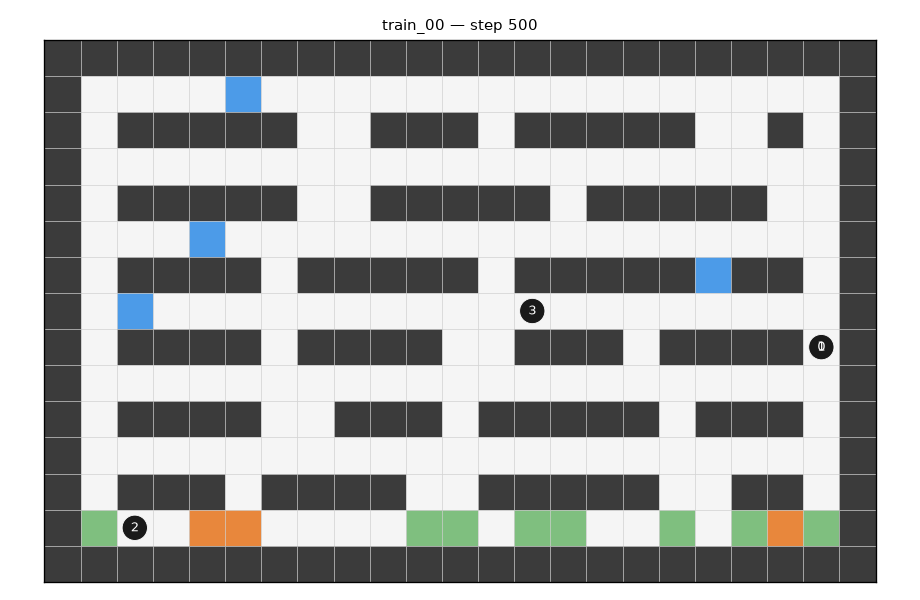
\includegraphics[width=0.6\textwidth]{figs/fig_demo_snapshot.png}
\caption{Снимок состояния симуляции, полученный
\code{save\_snapshot()} (файл \code{results/demo\_snapshot.png}): тёмные
окружности — роботы, подписанные своими номерами.}
\end{figure}

\begin{figure}[H]
\centering
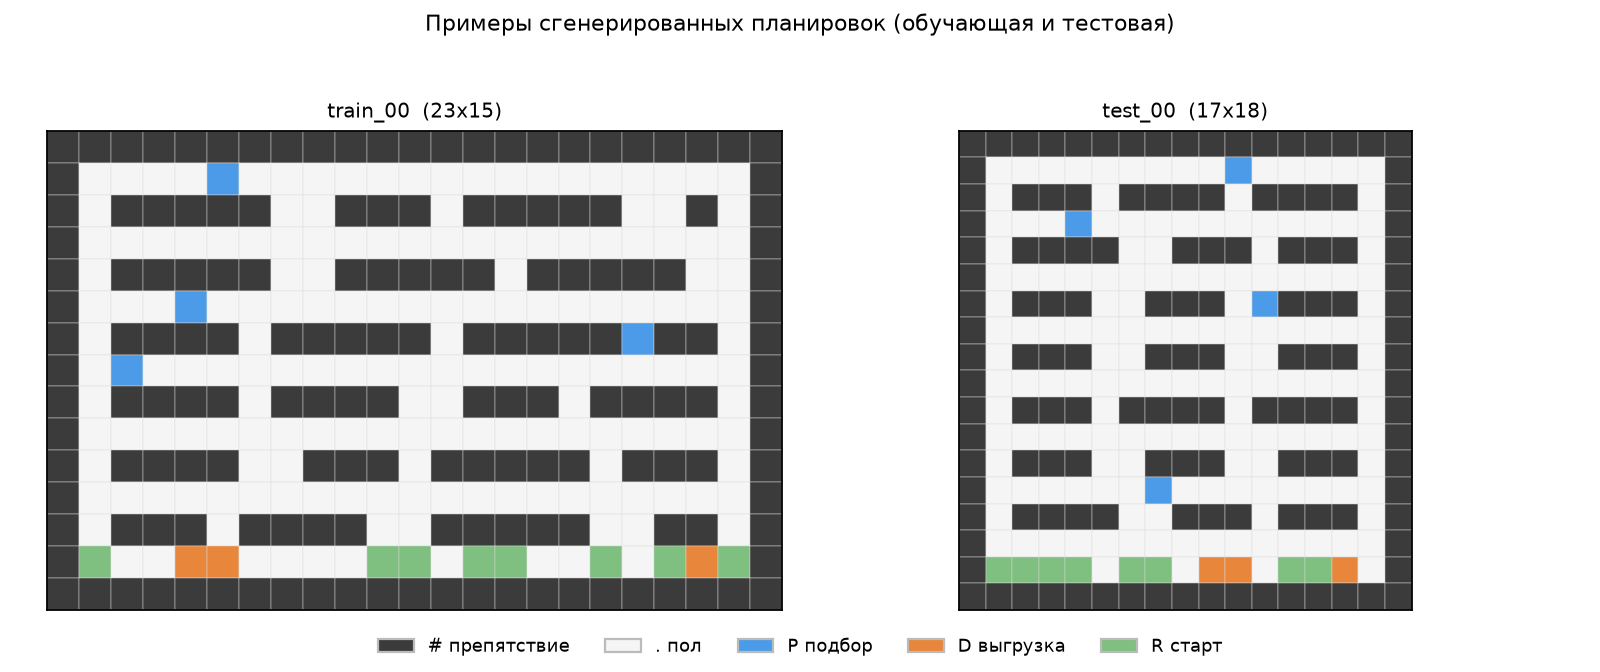
\includegraphics[width=0.98\textwidth]{figs/fig_layouts.png}
\caption{Примеры сгенерированных планировок: обучающая \code{train\_00} и
тестовая \code{test\_00}. Символы: \code{\#} — стеллаж, \code{.} — пол,
\code{P} — подбор, \code{D} — выгрузка, \code{R} — старт робота. Каждая
планировка проверяется генератором на полную связность.}
\end{figure}

% ============================================================================
\section{Навигация: A* и оракул расстояний}
% ============================================================================
Модуль \code{navigation/astar.py} решает классическую подзадачу движения по
статической сетке. Используется A* с допустимой эвристикой: манхэттенское
расстояние для 4-связности и октильное для 8-связности.

\begin{lstlisting}[style=py]
def _heuristic(a, b, connectivity):
    dr, dc = abs(a[0]-b[0]), abs(a[1]-b[1])
    if connectivity == 4:
        return float(dr + dc)
    return float(max(dr, dc) + (2.0**0.5 - 1.0) * min(dr, dc))   # октиль

def astar(walkable, start, goal, *, connectivity=4):
    """Минимальный по стоимости путь start..goal (включительно) или None."""
    ...
    return _reconstruct(came_from, current)
\end{lstlisting}

\code{DistanceOracle} кэширует пути и расстояния, поскольку планировка в течение
эпизода не меняется. Это делает жадный базлайн (который на каждом шаге
оценивает много пар робот--заказ) дешёвым. Расстояния симметричны, поэтому
один результат заполняет оба направления кэша.

\begin{lstlisting}[style=py]
class DistanceOracle:
    def path(self, start, goal):
        key = (start, goal)
        if key not in self._path_cache:
            self._path_cache[key] = astar(self.walkable, start, goal,
                                          connectivity=self.connectivity)
        return self._path_cache[key]

    def distance(self, start, goal):
        ...
        self._dist_cache[reverse] = value   # симметрия
        return value

    def reachable(self, start, goal):
        return self.distance(start, goal) is not None
\end{lstlisting}

% ============================================================================
\section{Алгоритмы распределения задач}
% ============================================================================
\subsection{Жадный базлайн (\code{greedy.py})}
Жадная политика — классическая неалгоритмическая точка отсчёта. Реализованы две
стратегии.

\begin{longtable}{@{}p{0.30\textwidth}p{0.64\textwidth}@{}}
\toprule
\textbf{Стратегия} & \textbf{Поведение} \\
\midrule
\endfirsthead
\toprule
\textbf{Стратегия} & \textbf{Поведение} \\
\midrule
\endhead
\code{min\_completion\_time} (по умолчанию) & Заказы обрабатываются от старых к
новым; каждому назначается свободный робот с наименьшим оценённым временем
завершения. \\
\code{nearest\_robot} & Каждому свободному роботу назначается ожидающий заказ с
ближайшим пунктом подбора. \\
\bottomrule
\end{longtable}

\begin{lstlisting}[style=py]
def estimate_completion_time(self, sim, robot, order):
    to_pickup = sim.oracle.distance(robot.position, order.pickup)
    if to_pickup is None:
        return None
    to_dropoff = sim.oracle.distance(order.pickup, order.dropoff)
    if to_dropoff is None:
        return None
    wcfg = sim.config.warehouse
    return to_pickup + wcfg.pick_dwell_steps + to_dropoff + wcfg.drop_dwell_steps

def _assign_min_completion_time(self, sim):
    pending = sim.pending_orders()          # от старых к новым
    available = {r.id for r in sim.idle_robots()}
    assignments = []
    for order in pending:
        best_robot, best_cost = None, float("inf")
        for robot_id in sorted(available):
            cost = self.estimate_completion_time(sim, sim.robots[robot_id], order)
            if cost is not None and cost < best_cost:
                best_cost, best_robot = cost, robot_id
        if best_robot is not None:
            assignments.append((best_robot, order.id))
            available.discard(best_robot)
    return assignments
\end{lstlisting}

Базлайн \emph{детерминирован} и, по замыслу, \textbf{никогда не настраивается}.
Авторы проекта не предполагают, что RL обязательно его превзойдёт.

\subsection{Заглушки PPO и DQN}
Файлы \code{ppo.py} и \code{dqn.py} определяют \emph{контракт интерфейса}
будущих политик (\code{assign}, \code{save}, \code{load}, атрибут \code{name}),
но конструкторы намеренно бросают \code{NotImplementedError}. Это делает
незавершённость явной вместо имитации обучения. Фабрика
\code{make\_policy(name, config)} возвращает \code{GreedyPolicy} для
\code{"greedy"} и бросает \code{NotImplementedError} для \code{"ppo"}/\code{"dqn"}.

% ============================================================================
\section{Метрики}
% ============================================================================
Модуль \code{metrics/metrics.py} собирает метрики на эпизод и агрегирует их.
Все времена — в шагах симуляции, расстояния — в единицах сетки.

\begin{longtable}{@{}p{0.38\textwidth}p{0.56\textwidth}@{}}
\toprule
\textbf{Метрика} & \textbf{Определение} \\
\midrule
\endfirsthead
\toprule
\textbf{Метрика} & \textbf{Определение} \\
\midrule
\endhead
Avg completion time & среднее \code{completed - created} \\
Avg waiting time & среднее \code{assigned - created} \\
Avg service time & среднее \code{completed - assigned} \\
Total travel distance & суммарное перемещение роботов (единицы сетки) \\
Throughput per 100 steps & завершённых заказов на 100 шагов \\
Robot utilization & занятые робото-шаги / (\code{n\_robots} $\times$ длительность) \\
\code{episode\_duration} & длительность эпизода в шагах \\
\code{n\_orders\_created} & создано заказов \\
\code{n\_orders\_completed} & завершено заказов \\
\code{n\_orders\_timed\_out} & истекло по таймауту \\
\code{n\_orders\_failed} & неуспешных (недостижимый участок) \\
\bottomrule
\end{longtable}

\begin{lstlisting}[style=py]
duration = int(sim.step_count)
n_completed = len(completed)
robot_steps = max(1, sim.n_robots * duration)

return EpisodeMetrics(
    layout=..., policy=..., seed=...,
    episode_duration=duration,
    n_orders_created=len(sim.orders),
    n_orders_completed=n_completed,
    avg_completion_time=_safe_mean(completion_times),
    avg_waiting_time=_safe_mean(waiting_times),
    avg_service_time=_safe_mean(service_times),
    total_travel_distance=float(sim.total_travel_distance),
    throughput_per_100_steps=(100.0 * n_completed / duration) if duration else 0.0,
    robot_utilization=float(sim.robot_busy_steps) / robot_steps,
)
\end{lstlisting}

Функции \code{records\_to\_rows}, \code{save\_records\_csv} пишут результаты в
CSV (через pandas, с запасным вариантом на стандартный \code{csv}).
\code{aggregate(records)} группирует метрики по \code{(policy, layout)} и
вычисляет \code{mean}/\code{std}.

% ============================================================================
\section{Экспериментальные сценарии}
% ============================================================================
\subsection{Обучение (\code{experiments/train.py})}
На текущей вехе обучение отсутствует: \code{train()} загружает обучающие
планировки, создаёт каталог запуска, сохраняет снимок конфигурации
(\code{config.yaml}) и пишет \code{MANIFEST.txt}. Для greedy это
<<no-op>>-обучение, а для \code{ppo}/\code{dqn} поднимается
\code{NotImplementedError} (каталог и снимок конфига при этом уже созданы).

\begin{lstlisting}[style=py]
def train(config, *, run_dir=None):
    layouts = load_training_layouts(config)
    run_dir = Path(run_dir) if run_dir else Path(config.output_dir) / config.algorithm
    run_dir.mkdir(parents=True, exist_ok=True)
    save_config(config, run_dir / "config.yaml")

    if config.algorithm == "greedy":
        policy = GreedyPolicy(config.greedy)
        (run_dir / "MANIFEST.txt").write_text(...)
        return TrainingResult(algorithm="greedy", policy=policy, ...)
    if config.algorithm in ("ppo", "dqn"):
        raise NotImplementedError(...)
    raise ValueError(f"Unknown algorithm '{config.algorithm}'")
\end{lstlisting}

\subsection{Оценка (\code{experiments/evaluate.py})}
Раннер оценки \emph{не зависит} от алгоритма. Эпизоды прогоняются по всем
планировкам, базовым сидам и повторам; для воспроизводимости и независимости
итоговый сид вычисляется как \code{base\_seed * 1\_000\_003 + episode}.

\begin{lstlisting}[style=py]
def evaluate_policy(policy, layouts, config, *, n_episodes=None, seeds=None, policy_name=None):
    n_episodes = n_episodes or config.n_episodes
    seeds = list(seeds) if seeds is not None else list(config.seeds)
    records = []
    for layout in layouts:
        for base_seed in seeds:
            for episode in range(n_episodes):
                ep_seed = int(base_seed) * SEED_STRIDE + episode
                records.append(run_episode(layout, config, policy,
                                           seed=ep_seed, policy_name=policy_name))
    return records
\end{lstlisting}

\subsection{Сравнение (\code{experiments/compare.py})}
\code{compare\_algorithms} прогоняет несколько политик на \emph{одних и тех же}
тестовых планировках и сидах, пишет \code{episodes.csv} и \code{summary.csv}, а
\code{summarize\_records} формирует сгруппированную сводку
(\code{mean}/\code{std} по политике). Это фундамент Эксперимента C.

% ============================================================================
\section{CLI-скрипты}
% ============================================================================
Все скрипты добавляют \code{src} в \code{sys.path}, поэтому работают без
установки пакета.

\begin{longtable}{@{}p{0.32\textwidth}p{0.60\textwidth}@{}}
\toprule
\textbf{Скрипт} & \textbf{Назначение} \\
\midrule
\endfirsthead
\toprule
\textbf{Скрипт} & \textbf{Назначение} \\
\midrule
\endhead
\code{generate\_layouts.py} & Генерация обучающих и тестовых наборов планировок
(по умолчанию 10+10). Флаг \code{--force} для перегенерации. \\
\code{train.py} & Запуск <<обучения>> (для greedy — создание артефактов запуска). \\
\code{evaluate.py} & Оценка политики на тестовых планировках, вывод сводки,
запись CSV. \\
\code{demo.py} & Сквозное демо: один эпизод greedy, ASCII-кадры, PNG-снимок,
опционально GIF. \\
\bottomrule
\end{longtable}

\begin{lstlisting}[style=plain]
# 1) Сгенерировать планировки
python scripts/generate_layouts.py
# 2) Демо: один greedy-эпизод + снимок
python scripts/demo.py --every 100 --snapshot results/demo.png
# 3) Оценка greedy на тестовых планировках
python scripts/evaluate.py --episodes 3
# 4) <<Обучение>> (greedy — no-op)
python scripts/train.py
# 5) Тесты
python -m pytest
\end{lstlisting}

% ============================================================================
\section{Тесты}
% ============================================================================
Тестовый набор содержит \textbf{40 тестов} pytest
(\code{tests/}), покрывающих четыре области.

\begin{longtable}{@{}p{0.34\textwidth}cp{0.50\textwidth}@{}}
\toprule
\textbf{Файл} & \textbf{Тестов} & \textbf{Проверяемое} \\
\midrule
\endfirsthead
\toprule
\textbf{Файл} & \textbf{Тестов} & \textbf{Проверяемое} \\
\midrule
\endhead
\code{test\_config.py} & 8 & Загрузка конфигов, extends, dotted-overrides,
ошибки типов, save/reload. \\
\code{test\_layouts.py} & 12 & Валидация планировок, детерминизм генерации,
связность, непересекаемость train/test. \\
\code{test\_environment.py} & 11 & Сквозные эпизоды, детерминизм, reset,
валидация назначений, таймауты, метрики. \\
\code{test\_navigation.py} & 9 & A*: кратчайшие пути, обход препятствий,
8-связность, кэш и симметрия оракула. \\
\bottomrule
\end{longtable}

Тесты подтверждают ключевые инварианты: политика назначает только свободных
роботов на ожидающие заказы; один робот получает не более одного заказа за шаг;
эпизод детерминирован при одинаковом сиде; при недостижимом пункте подбора
заказ пропускается.

% ============================================================================
\section{Конфигурационные файлы и артефакты}
% ============================================================================
\subsection{Конфигурации}
\code{default.yaml} задаёт базовые параметры: размеры сетки, число роботов,
времена сервиса, горизонт эпизода, скорость, связность, интервал решений, поток
заказов, размеры наборов планировок, стратегию greedy и заглушку reward.
\code{training.yaml} и \code{evaluation.yaml} подключают его через
\code{extends: default.yaml} и добавляют специфичные поля.

\begin{center}
\begin{tabular}{@{}ll@{}}
\toprule
\textbf{Параметр} & \textbf{Значение по умолчанию} \\
\midrule
\code{warehouse.n\_robots} & 4 \\
\code{warehouse.max\_steps} & 500 \\
\code{warehouse.connectivity} & 4 \\
\code{warehouse.decision\_interval} & 1 \\
\code{orders.arrival\_rate} & 0.35 \\
\code{orders.max\_pending} & 25 \\
\code{layout.n\_train / n\_test} & 10 / 10 \\
\code{layout.generation\_seed} & 20240101 \\
\code{greedy.strategy} & min\_completion\_time \\
\bottomrule
\end{tabular}
\end{center}

\subsection{Артефакты результатов}
\begin{itemize}[nosep]
\item \code{results/evaluation/greedy\_episodes.csv} — 60 эпизодных записей
(10 тестовых планировок $\times$ 3 базовых сида $\times$ 2? — фактически 6
запусков на планировку).
\item \code{results/evaluation/} — каталог для CSV оценки.
\item \code{results/training/greedy/} — снимок конфигурации
(\code{config.yaml}) и \code{MANIFEST.txt} для запуска greedy.
\item \code{results/demo\_snapshot.png} — иллюстративный снимок симуляции.
\end{itemize}

% ============================================================================
\section{Результаты базовой оценки (greedy)}
% ============================================================================
По имеющемуся CSV (\code{greedy\_episodes.csv}) вычислены средние значения по 60
эпизодам (10 тестовых планировок, 6 повторов каждая). Все планировки
завершались за фиксированный горизонт 500 шагов.

\begin{center}
\begin{tabular}{@{}lrr@{}}
\toprule
\textbf{Метрика (по эпизодам)} & \textbf{Среднее} & \textbf{Ст. отклонение} \\
\midrule
Avg completion time           & 137.70 & 18.48 \\
Avg waiting time              & 110.57 & 14.55 \\
Avg service time              & 27.13  & 4.13 \\
Total travel distance         & 1694.55 & 44.89 \\
Throughput per 100 steps      & 13.95  & 2.25 \\
Robot utilization             & 0.954  & 0.006 \\
Заказов создано               & 97.97  & 10.97 \\
Заказов завершено             & 69.73  & 11.24 \\
\bottomrule
\end{tabular}
\end{center}

Всего в наборе завершено 4184 заказа; \code{n\_orders\_timed\_out} и
\code{n\_orders\_failed} равны нулю (таймауты по умолчанию отключены,
недостижимых участков нет). Утилизация роботов очень высока ($\approx$95\%),
что указывает на достаточную загрузку при \code{arrival\_rate=0.35} и 4 роботах.
Эти числа — точка отсчёта для будущих RL-политик, а не утверждение о
превосходстве.

\subsection{Временные метрики по планировкам}
Рисунок~\ref{fig:times} показывает, что порядок величин устойчив: время
\emph{ожидания} доминирует над временем \emph{обслуживания} примерно в 4 раза.
Это ожидаемо: робот получает заказ не мгновенно после его появления, а по
решению политики; большая часть lead time — это пребывание заказа в очереди.

\begin{figure}[H]
\centering
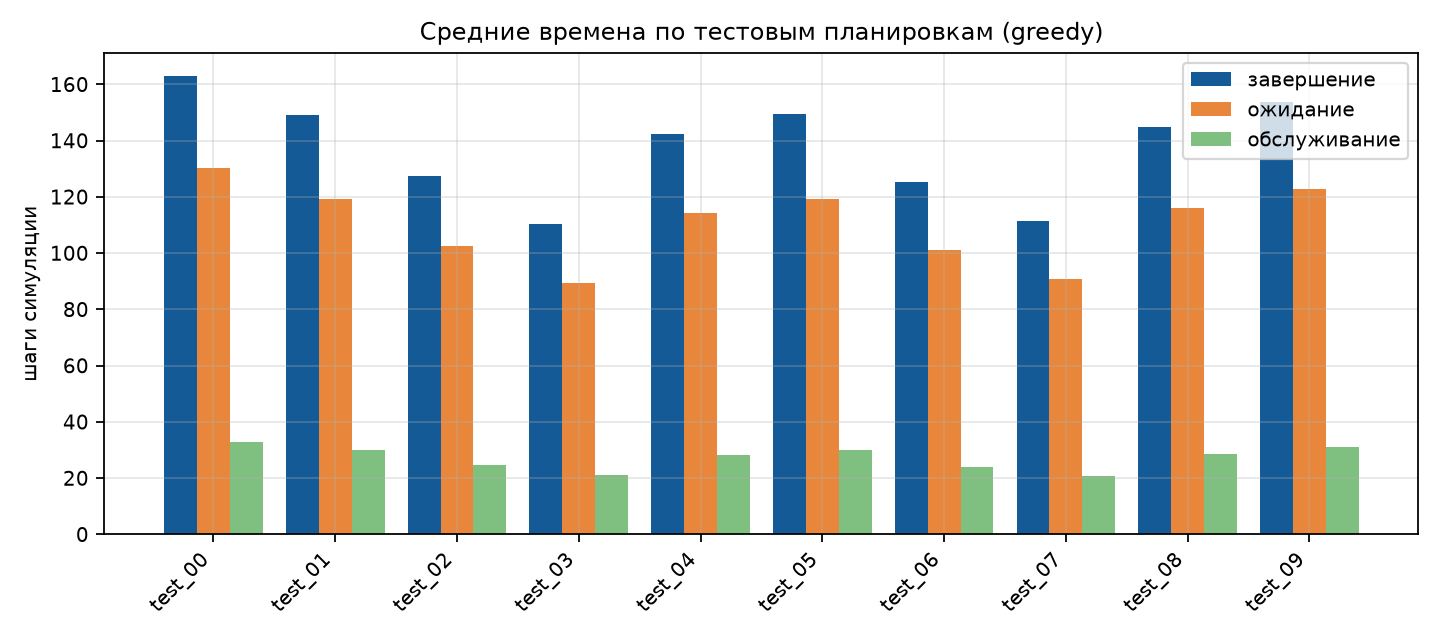
\includegraphics[width=0.95\textwidth]{figs/fig_times_by_layout.png}
\caption{Средние времена (завершение, ожидание, обслуживание) по каждой из 10
тестовых планировок. Планировки \code{test\_03} и \code{test\_07} дают
наименьшее время завершения, \code{test\_00}, \code{test\_05}, \code{test\_09} —
наибольшее.}
\label{fig:times}
\end{figure}

\subsection{Производительность и загрузка}
На рисунке~\ref{fig:thru} видна обратная связь производительности с размером
времени завершения: планировки с высокой пропускной способностью
(\code{test\_03}, \code{test\_07}) имеют и наименьшее время завершения.
Утилизация роботов всюду держится в диапазоне $0.94$--$0.96$, то есть роботы
почти не простаивают при \code{arrival\_rate=0.35} и 4 роботах.

\begin{figure}[H]
\centering
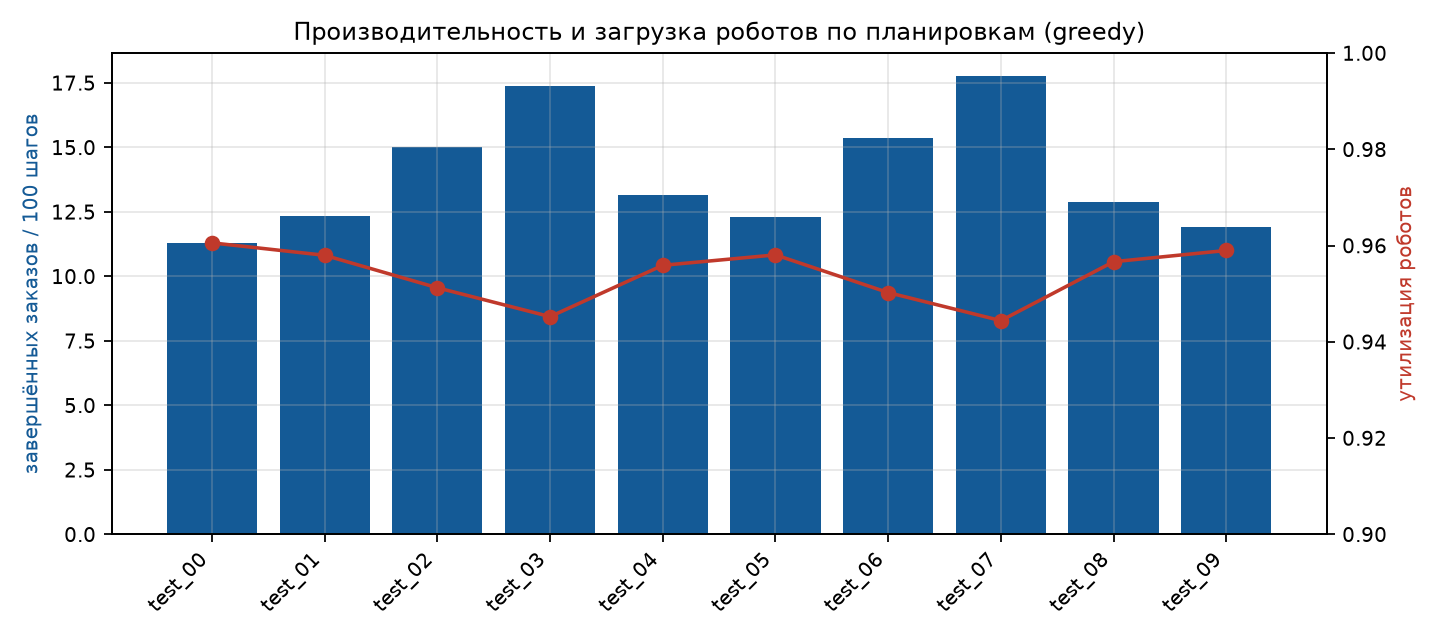
\includegraphics[width=0.95\textwidth]{figs/fig_throughput_util.png}
\caption{Пропускная способность (столбцы, левая ось) и утилизация роботов
(линия, правая ось) по тестовым планировкам.}
\label{fig:thru}
\end{figure}

\subsection{Разброс и корреляции}
Рисунок~\ref{fig:box} показывает распределение временных метрик по всем 60
эпизодам: медианы близки к средним, выраженных выбросов нет.
Рисунок~\ref{fig:scatter} отображает связь пройденной дистанции и
производительности: точки группируются по планировкам, и рост дистанции не
приводит к росту пропускной способности — то есть более <<далёкие>> планировки
просто тратят больше перемещений на тот же объём работы.

\begin{figure}[H]
\centering
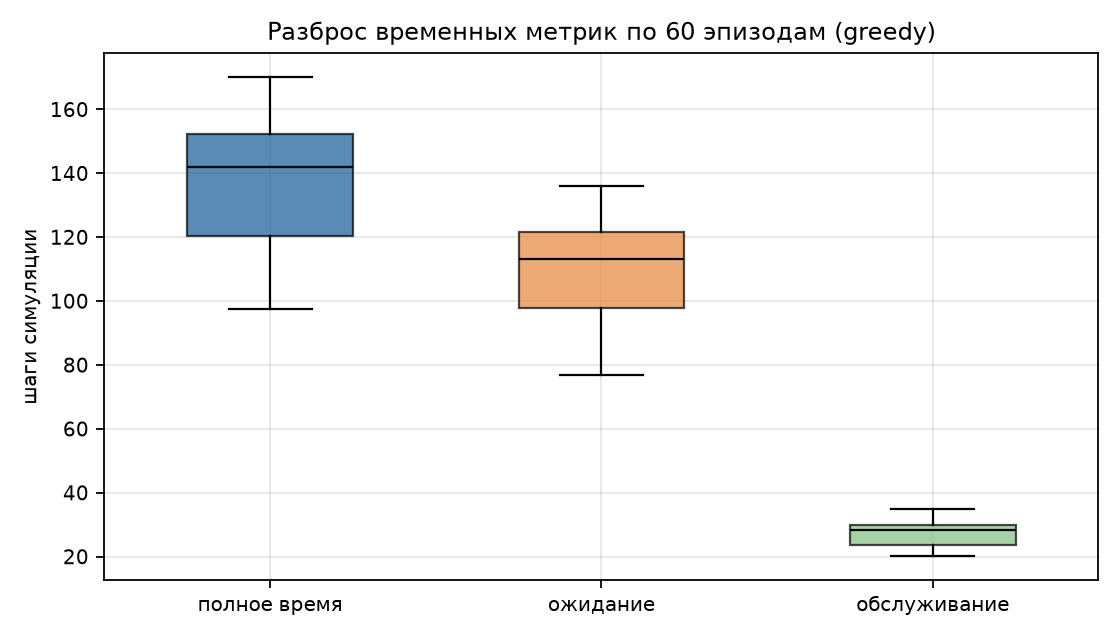
\includegraphics[width=0.72\textwidth]{figs/fig_box_times.png}
\caption{Разброс временных метрик по 60 эпизодам.}
\label{fig:box}
\end{figure}

\begin{figure}[H]
\centering
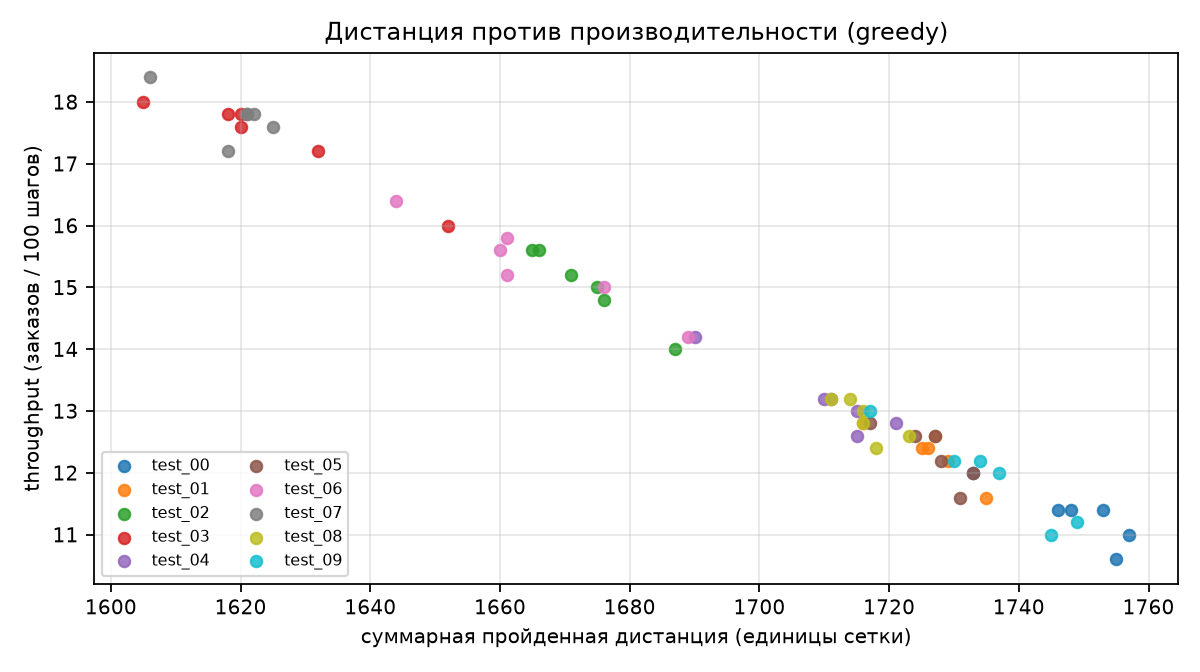
\includegraphics[width=0.82\textwidth]{figs/fig_travel_throughput.png}
\caption{Суммарная пройденная дистанция против пропускной способности; цвет
соответствует тестовой планировке.}
\label{fig:scatter}
\end{figure}

\begin{tcolorbox}[colback=accent!5,colframe=accent!60,title=Интерпретация]
Различия между планировками (пропускная способность от $\approx$11 до
$\approx$18 заказов/100 шагов) — это \emph{именно} тот сигнал, который должно
учитывать исследование обобщения. Обучаясь на 10 планировках и тестируясь на 10
невиданных, RL-политика должна показать, что она не <<переобучилась>> под
конкретную геометрию, а выучила переносимую стратегию распределения.
\end{tcolorbox}

% ============================================================================
\section{Замечания по коду и наблюдения}
% ============================================================================
Анализ выявил несколько неблокирующих моментов, полезных для развития проекта:
\begin{itemize}[nosep]
\item В \code{astar()} модуль \code{heapq} импортируется \emph{внутри} цикла
поиска — стоит вынести импорт на уровень модуля (микрооптимизация).
\item В \code{compute\_episode\_metrics} поле \code{n\_orders\_created}
вычисляется как \code{len(sim.orders)}, хотя в симуляции уже ведётся счётчик
\code{n\_orders\_created}. Оба эквивалентны, поскольку заказы из словаря не
удаляются, но дублирование стоит устранить.
\item CSV-файл результатов содержит колонку \code{orders\_per\_completed}, которой
\emph{нет} в текущем dataclass \code{EpisodeMetrics}. Похоже, файл создан более
ранней версией схемы метрик — стоит перегенерировать артефакты либо добавить
миграцию.
\item \code{results/**} исключён в \code{.gitignore} (кроме \code{.gitkeep}),
однако в репозитории присутствуют закоммиченные примеры
(\code{greedy\_episodes.csv}, снимки, артефакты greedy). Стоит унифицировать
политику хранения артефактов.
\item \code{RewardConfig} пока не используется — это заготовка под
Gymnasium-обёртку (веха M3).
\item Такие же заглушки \code{ppo.py}/\code{dqn.py} явно и честно сигнализируют
о незавершённости через \code{NotImplementedError}.
\end{itemize}

% ============================================================================
\section{Ограничения, допущения и дорожная карта}
% ============================================================================
\subsection{Сознательные упрощения}
\begin{itemize}[nosep]
\item Роботы \emph{не избегают} столкновений (клетки могут совпадать).
Бесконфликтное движение — будущая работа; на исследовательский вопрос о
\emph{распределении} оно не влияет.
\item Эпизод имеет \emph{фиксированный горизонт} (\code{max\_steps});
\code{done == truncated}.
\item \code{timeout\_steps} истекает только для \emph{неназначенных} заказов.
\item Жадный базлайн детерминирован и \emph{не} настраивается.
\end{itemize}

\subsection{Репродуктивность и научная честность}
Число роботов, размеры склада, число планировок и все сиды задаются
конфигурацией. Обучающие/тестовые планировки берутся из \emph{непересекающихся}
потоков сидов. Один и тот же тестовый набор и сиды используются для всех
сравниваемых алгоритмов. Снимки конфигураций и сырые CSV сохраняются
автоматически. Никаких <<прошитых>> результатов нет — оценка каждый раз
прогоняет симулятор с нуля.

\subsection{Дорожная карта}
\begin{center}
\begin{tabular}{@{}clc@{}}
\toprule
\textbf{Веха} & \textbf{Содержание} & \textbf{Статус} \\
\midrule
M1 & Сетка, роботы, поток заказов, A*, рендеринг & Готово \\
M2 & Greedy-базлайн, проверка завершения заказов, метрики & Готово \\
M3 & Обёртка Gymnasium (observation/action/reward) & Следующая \\
M4 & Обучение PPO на одной планировке, save/reload, оценка & Ожидается \\
M5 & Обучение на $N$ планировках $\rightarrow$ оценка на невиданных & Ожидается \\
M6 & PPO vs greedy (+ DQN при практичности) по размеру набора & Ожидается \\
\bottomrule
\end{tabular}
\end{center}

Запланированы три эксперимента: A (обучение на 10, тест на невиданных),
B (размер обучающего набора $1/3/5/10$ на фиксированном тесте),
C (greedy vs PPO vs опционально DQN).

% ============================================================================
\section{Установка и запуск}
% ============================================================================
Требуется Python $\geq$ 3.10. Рекомендуется \code{uv}:

\begin{lstlisting}[style=plain]
uv venv --python 3.14 .venv
uv pip install -e ".[dev,analysis]"   # ядро + pytest + pandas + matplotlib
uv pip install -e ".[rl]"             # стек RL (PyTorch, SB3, gymnasium) - тяжёлый
\end{lstlisting}

\begin{center}
\begin{tabular}{@{}lll@{}}
\toprule
\textbf{Extra} & \textbf{Зависимости} & \textbf{Назначение} \\
\midrule
(ядро) & numpy, pyyaml & симулятор + greedy (M1--M2) \\
\code{rl} & gymnasium, torch, stable-baselines3 & обучение RL (M4--M6) \\
\code{analysis} & pandas, matplotlib & анализ и графики \\
\code{dev} & pytest & тесты \\
\bottomrule
\end{tabular}
\end{center}

% ============================================================================
\section{Краткий API-справочник}
% ============================================================================
\begin{longtable}{@{}p{0.44\textwidth}p{0.50\textwidth}@{}}
\toprule
\textbf{Символ} & \textbf{Описание} \\
\midrule
\endfirsthead
\toprule
\textbf{Символ} & \textbf{Описание} \\
\midrule
\endhead
\code{load\_config(path, config\_cls, overrides)} & Загрузка YAML в dataclass. \\
\code{save\_config(config, path)} & Сохранение снимка конфигурации. \\
\code{Layout.read / write / is\_connected} & Чтение, запись и проверка
связности планировки. \\
\code{generate\_layout / generate\_layout\_suite} & Генерация одной планировки /
набора. \\
\code{generate\_train\_test\_suites} & Генерация и сохранение train/test. \\
\code{OrderGenerator.maybe\_generate(step, pending\_count)} & Поток заказов. \\
\code{WarehouseSimulation(layout, config, seed)} & Создание симуляции. \\
\code{sim.step / sim.run / sim.reset} & Управление эпизодом. \\
\code{sim.assign / can\_assign} & Валидация и назначение заказа роботу. \\
\code{sim.ascii\_render} & ASCII-снимок состояния. \\
\code{astar / DistanceOracle} & Планирование пути и кэш расстояний. \\
\code{GreedyPolicy.assign / make\_policy} & Политика и фабрика. \\
\code{evaluate\_policy / evaluate\_from\_config} & Оценка политики. \\
\code{compare\_algorithms / summarize\_records} & Сравнение и сводка. \\
\code{train / train\_from\_config} & Раннер обучения. \\
\code{compute\_episode\_metrics / save\_records\_csv} & Метрики и экспорт. \\
\bottomrule
\end{longtable}

\vfill
\begin{tcolorbox}[colback=accent!5,colframe=accent!60]
\textbf{Итог.} Репозиторий \code{RRS} — это аккуратно структурированный
исследовательский фреймворк на вехах M1--M2: полностью реализованы и покрыты
тестами симулятор, навигация A*, генерация планировок, жадный базлайн,
конфигурация и метрики. RL-часть (M3--M6) корректно оставлена в виде явных
заглушек с описанным контрактом интерфейса. Архитектура сознательно разделяет
\emph{распределение задач} (изучается RL) и \emph{навигацию} (классический A*),
что и позволяет строго изучать обобщение политик на невиданные планировки.
\end{tcolorbox}

\end{document}
